\documentclass[11pt,letterpaper]{article}
% Standalone companion to the frozen baseline model and reference notes.
\usepackage[margin=1in]{geometry}
\usepackage[T1]{fontenc}
\usepackage{lmodern}
\usepackage{amsmath,amssymb,mathtools}
\usepackage{graphicx,microtype,booktabs,array,tabularx}
\usepackage{enumitem,xcolor,parskip}
\usepackage[most]{tcolorbox}
\usepackage{hyperref,titlesec,caption,fancyhdr,listings}
\hypersetup{colorlinks=true,linkcolor=blue!40!black,urlcolor=blue!60!black,
 pdftitle={A Simplified Dual-Oscillator Model of Seasonal Transcriptional Timing},
 pdfauthor={Shanshan Qin},pdfsubject={Model reduced model: symmetric PDF drive and mean-gap dynamics}}
\titleformat{\section}{\Large\bfseries\color{blue!40!black}}{\thesection}{1em}{}
\titleformat{\subsection}{\large\bfseries\color{blue!50!black}}{\thesubsection}{1em}{}
\titlespacing*{\section}{0pt}{1.1\baselineskip}{0.4\baselineskip}
\titlespacing*{\subsection}{0pt}{0.8\baselineskip}{0.3\baselineskip}
\captionsetup{font=small,labelfont=bf}
\setlist{leftmargin=*,itemsep=2pt,topsep=3pt}
\newcommand{\pdfzero}{\textit{pdf}\textsuperscript{0}}
\newcommand{\relu}[1]{\left[#1\right]_+}
\newcommand{\wrap}{\operatorname{wrap}_{24}}
\newcolumntype{Y}{>{\raggedright\arraybackslash}X}
\lstset{basicstyle=\ttfamily\footnotesize,breaklines=true,columns=fullflexible,
 keepspaces=true,frame=single,rulecolor=\color{black!15},backgroundcolor=\color{black!2}}
\pagestyle{fancy}
\fancyhf{}
\fancyhead[L]{\small Seasonal transcriptional timing}
\fancyhead[R]{\small Model reduced model: simplification study}
\fancyfoot[C]{\thepage}
\setlength{\headheight}{14pt}
\renewcommand{\headrulewidth}{0.3pt}
\fancypagestyle{plain}{\fancyhf{}\fancyfoot[C]{\thepage}\renewcommand{\headrulewidth}{0pt}}
\raggedbottom

\title{\textbf{A Simplified Dual-Oscillator Model of\\
Seasonal Transcriptional Timing in \textit{Drosophila}}\\[6pt]
\large Version 0.3: symmetric PDF drive and mean--gap dynamics}
\author{Shanshan Qin}
\date{9 October 2026}

\begin{document}
\maketitle

\begin{tcolorbox}[colback=blue!3,colframe=blue!30!black,boxrule=0.6pt,
 title=Purpose and main result]
The ten-parameter reference model can be reduced to seven free clock parameters
by sharing the M/E PDF strength, removing the release offset, and setting
the release-window exponent to one. Its paired WT peak-time RMSE remains
$0.229$\,h, compared with $0.231$\,h for reference model.
Fixing three additional, data-informed constants gives a four-parameter
alternative with the same all-data phase predictions in this search.
Both pass the tested long-run entrainment audit and retain similar
raw-waveform agreement after refitting. The symmetric formulation also
separates mean timing from the M--E phase difference.
\end{tcolorbox}

\section{Scope and recommendation}

This note is a standalone account of the reduced model simplification study.
The experimental targets are \textit{tim} transcriptional peaks in
morning (M; sLNv) and evening (E; fifth sLNv) neurons, measured across
11 photoperiods, plus PDF/PDFR perturbations and an LD-to-DD transfer
\cite{project}. The reference model baseline and its report remain preserved
\cite{v02}.

\begin{center}
\small
\begin{tabular}{lrrr}
\toprule
Model & Free clock parameters & WT RMSE (h) & Conditional CV (h)\\
\midrule
Reference model & 10 & 0.231 & 0.249\\
reduced model symmetric, linear release & 7 & 0.229 & 0.241\\
reduced model with fixed reference constants & 4 & 0.229 & 0.240\\
\bottomrule
\end{tabular}
\end{center}

The \textbf{seven-parameter formulation is the conservative recommendation}.
It removes three fitted freedoms while retaining estimation of the
short-day reference and activation scale. The four-parameter formulation
is useful as a compact phenomenological model, provided its additional
fixed constants are stated explicitly. Neither the small error differences
nor conditional cross-validation establish superior prediction.

The implementation is distributed as the manuscript code release.
This report does not promote the candidate to a mechanistically validated
model or freeze a new release. The interpretation remains an effective
description of stationary photoperiod responses; DD4 common timing,
light-pulse responses, amplitude dynamics, and causal daylength sensing
remain unresolved.

\clearpage
\section{The seven-parameter formulation}
\label{sec:model}

Each neuron population has an unwrapped phase $\phi_i$, with a
transcriptional peak at $\phi_i=\pi\pmod{2\pi}$.
For photoperiod $P$ in hours, $L(t)=1$ when $(t\bmod24)<P$ and zero
otherwise. All dynamical gains below are nonnegative.
Define $\omega=2\pi/24$\,rad/h and
\begin{align}
P_c&=\min(P,15),\quad x=\max(0,P_c-9),\quad
F(P)=\frac{x^2}{x^2+h_P^2},\label{eq:F}\\
B(P)&=\max(P_f,P_c)+\lambda_s+(\lambda-\lambda_s)F(P),\label{eq:B}\\
\theta(t;P)&=\omega t+\pi-\omega B(P),\notag\\
S(t;P)&=L(t)\relu{\cos\theta(t;P)}F(P).\label{eq:S}
\end{align}
The inherited 9-hour onset, 15-hour cap, and activation exponent 2
are fixed empirical rules. The exponent removed from reference belongs
to the positive-cosine \emph{release window}, not to $F$.

The simplified phase equations are
\begin{equation}
\boxed{\begin{aligned}
\dot\phi_M&=\omega+KL\sin(\theta-\phi_M)
                  +\kappa\sin(\phi_E-\phi_M)+g_M\gamma S,\\
\dot\phi_E&=\omega+KL\sin(\theta-\phi_E)
                  -\kappa\sin(\phi_E-\phi_M)-g_E\gamma S.
\end{aligned}}\label{eq:phase}
\end{equation}
Here $K$ attracts each phase toward a shared rotating light reference,
$\gamma$ gives the effective PDF-associated separating drive, and
$\kappa$ supplies symmetric synchronization. Coupling is retained in
PDF-null and receptor-loss simulations; its biological mediator is
not identified. The flags $(g_M,g_E)$ are $(1,1)$ in WT, $(0,0)$ in
\pdfzero{}, $(0,1)$ for M-specific PDFR loss, and $(1,0)$ for
E-specific PDFR loss.

Relative to reference, $\alpha=\beta=\gamma$, $\chi=0$ and $q=1$.
Release remains tied to the common reference rather than to
$\phi_M$. The fit does not measure PDF secretion or establish its
coincidence with transcription.

\begin{table}[!htbp]
\centering\scriptsize
\setlength{\tabcolsep}{3.5pt}
\renewcommand{\arraystretch}{1.15}
\begin{tabularx}{\textwidth}{lrrrlY}
\toprule
 & Phase fit & Raw fit: 7 & Raw fit: 4 & Units & Meaning\\
\midrule
$K$ & 0.072934 & 0.071535 & 0.065458 & rad/h & Shared light attraction \\
$\lambda$ & 3.008976 & 2.678316 & 2.671647 & h & Long-day reference lag \\
$\gamma$ & 0.108250 & 0.116797 & 0.106642 & rad/h & Common PDF strength \\
$\kappa$ & 0.006216 & 0.007097 & 0.006709 & rad/h & Synchronizing coupling \\
$h_P$ & 1.000000 & 1.011671 & 1.000000 & h & Activation half-scale \\
$P_f$ & 7.000000 & 7.017425 & 7.000000 & h & Short-day floor \\
$\lambda_s$ & 1.000000 & 0.928589 & 1.000000 & h & Short-day lag
\\
\bottomrule
\end{tabularx}
\caption{Parameters of the symmetric formulation. The phase-fit values
coincide for the seven- and four-parameter candidates in the saved search.
In the four-parameter model, $h_P=1$, $P_f=7$ and $\lambda_s=1$ are fixed.
Raw fits are distinct presets. Display precision is not a confidence interval.}
\label{tab:params}
\end{table}

\clearpage
\section{An exact mean--gap representation}
\label{sec:mean}

Define mean phase and signed phase difference by
\begin{equation}
m=\frac{\phi_M+\phi_E}{2},\qquad
\delta=\phi_E-\phi_M,\qquad
\phi_M=m-\frac{\delta}{2},\quad \phi_E=m+\frac{\delta}{2}.
\end{equation}
Individual phases admit equivalent lifts differing by $2\pi$.
WT orbit comparisons below choose lifts with $|\delta|<\pi$;
shifting one phase by $2\pi$ also shifts $m$ by $\pi$.
Adding and subtracting Eq.~\eqref{eq:phase} gives
\begin{equation}
\boxed{\begin{aligned}
\dot m&=\omega+KL\sin(\theta-m)\cos(\delta/2)
                 +(g_M-g_E)\gamma S/2,\\
\dot\delta&=-2KL\cos(\theta-m)\sin(\delta/2)
                 -2\kappa\sin\delta-(g_M+g_E)\gamma S.
\end{aligned}}\label{eq:mean}
\end{equation}
These equations are exact within the unclamped domain below.
They are not a small-angle approximation. A 4--5\,h peak gap corresponds
to phase differences of order 1 rad, so replacing all sine terms by
linear terms is not uniformly justified.

\subsection{Why the nonnegative-velocity clamp can be removed}

The reference equations apply $\max(0,\cdot)$ to each phase velocity.
Under binary light, $0\leq S\leq1$, and
\begin{equation}
\dot\phi_i\geq \omega-K-\gamma-\kappa>0.
\label{eq:bound}
\end{equation}
At the reduced model phase preset, the lower bound is $0.074400$\,rad/h.
The clamp is therefore idle for every phase and photoperiod, including
the tested knockout flags. Its removal introduces no new approximation.
The compact implementation requires $K+\gamma+\kappa<\omega$ and rejects
nonbinary intensity inputs. Equation~\eqref{eq:bound} is not a claim
about high-intensity pulses or arbitrary strong-drive parameters.

\subsection{One state is sufficient on the entrained WT orbit}

In WT the PDF terms cancel in $\dot m$.
For constant $P$, set $u=m-\theta$; then
\begin{equation}
\dot u=-KL\sin u\cos(\delta/2).
\end{equation}
The orbit $u=0$ is invariant. It attracts small deviations if
$|\delta|<\pi$ and repeated light exposure persists. On that orbit,
the remaining WT dynamics are
\begin{equation}
\dot\delta=-2KL\sin(\delta/2)-2\kappa\sin\delta-2\gamma S.
\label{eq:scalar}
\end{equation}
This makes the roles clearer: the reference fixes mean phase, while
separating PDF drive competes with synchronization to shape the gap.
General initial conditions and receptor-loss transients still require
both states. Mean phase is not generally the arithmetic mean of the two
peak times; those peaks occur at different times during evolving $\delta$.
A positive E-minus-M peak-time gap corresponds to negative $\delta$,
and equals approximately $-\delta/\omega$ only when $\delta$ changes slowly.

\clearpage
\section{The compact four-parameter alternative}

Fixing $P_f=7$\,h, $\lambda_s=1$\,h and $h_P=1$\,h leaves only
$(K,\lambda,\gamma,\kappa)$ free. The reference becomes
\begin{equation}
F(P)=\frac{x^2}{x^2+(1\,\mathrm{h})^2},\qquad
B(P)=\max(8\,\mathrm{h},P_c+1\,\mathrm{h})
                   +(\lambda-1\,\mathrm{h})F(P).
\label{eq:four}
\end{equation}
Equations~\eqref{eq:S} and \eqref{eq:mean} otherwise remain unchanged.
The rounded constants are suggested by the existing fits and short-day
observations. They are not independent measurements. The free-parameter
count does not include the data-informed reference form and landmarks.

\begin{figure}[h]
\centering
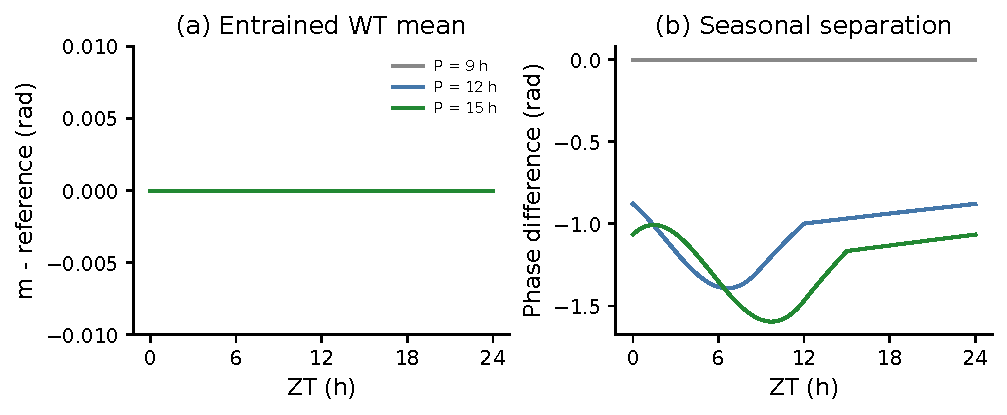
\includegraphics[width=\textwidth]{figure/report/mean_and_gap.pdf}
\caption{The compact phase preset after 60 days of constant LD.
The entrained WT mean follows $\theta$, while $\delta$ changes with
photoperiod and within the day. Curves use $P=9$, 12 and 15\,h;
the P=9 gap is zero because $F=0$. The small mean-axis range exposes
numerical deviations around the invariant orbit. Equivalent phase lifts
remove relative $2\pi$ winding before plotting $m$ and $\delta$.}
\label{fig:mean}
\end{figure}

The independent mean--gap integrator was compared with the constrained
reference phase integrator at all 11 WT photoperiods and the three LD12
knockout conditions. All 14 compact solutions locked.
The maximum peak discrepancy was $0.004465$\,h; the maximum DD gap
discrepancy was $0.006049$\,h. These differences are consistent with
the numerical integration and peak interpolation tolerances used.

The module \texttt{code/phase\_model.py} implements this
four-parameter core. The seven-parameter candidate uses the same
equations through a constrained fitting workflow; its saved results are
supplied with this distribution.

\begin{tcolorbox}[colback=black!2,colframe=black!60,boxrule=0.5pt,
 title=What has and has not been simplified]
The three reductions from ten to seven remove fitted freedoms.
The additional reduction to four fixes three constants using the data.
The WT scalar equation reduces state dimension on an invariant orbit;
it does not eliminate the second population or replace knockout
and transient simulations.
\end{tcolorbox}

\clearpage
\section{Seasonal and knockout agreement}

\begin{figure}[h]
\centering
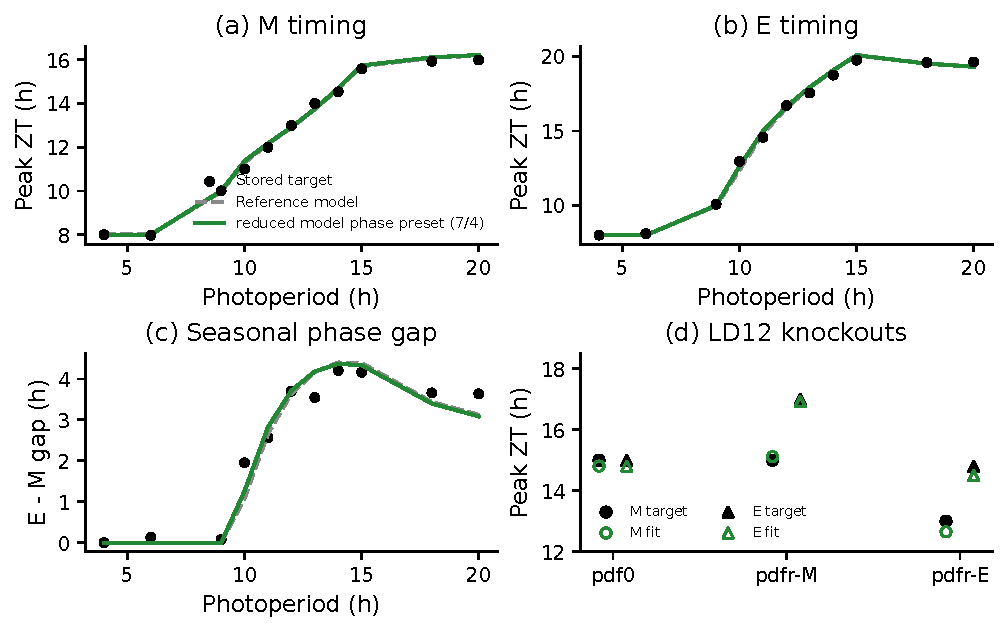
\includegraphics[width=\textwidth]{figure/report/seasonal_fit.pdf}
\caption{Saved phase fits compared with the stored paired WT estimates.
The seven- and four-parameter candidates have identical all-data
predictions in this local search and are shown by one green curve.
The grey dashed curves are reference model. The gap is derived from the
two peak times, not fitted as an additional independent datum.
Knockout markers compare LD12 targets with stationary predictions.
Small horizontal marker offsets distinguish M/E; they do not represent
different experimental conditions.}
\label{fig:seasonal}
\end{figure}

\begin{table}[!htbp]
\centering\small
\begin{tabular}{lrrrr}
\toprule
LD12 condition & M target & E target & M fit & E fit\\
\midrule
\pdfzero{} & 15.0 & 15.0 & 14.808 & 14.808 \\
M-specific PDFR loss & 15.0 & 17.0 & 15.116 & 16.915 \\
E-specific PDFR loss & 13.0 & 14.8 & 12.653 & 14.507
\\
\bottomrule
\end{tabular}
\caption{Stationary peak times in ZT hours for the shared reduced model phase preset.
The \pdfzero{} common peak contributes once to the fitting objective.
The targets use the inherited 0.5\,h calibration scale.}
\end{table}

All six phase-fit reductions and both raw-fit reductions pass the
80-day orbit audit: WT $P=4,\ldots,20$\,h and all three LD12 knockout
conditions, each from three distinct initial phase pairs.
Locking requires one peak crossing per day, rotation within 0.005 cycles
of one cycle/day, and day-to-day peak drift below 0.05\,h.
For the four-parameter phase preset, maximum audited drift is
0.00367\,h and maximum initial-condition peak difference is 0.00425\,h.
These checks demonstrate convergence for the tested cases, not global
stability for every parameter or stimulus.

Seasonal fits are stationary approximations: WT measurements were taken
after LD7 and knockout measurements after LD4. Actual experimental
initial phases were unavailable, so the fitting study does not directly
reproduce those finite-duration starting protocols.

\clearpage
\section{Controlled reduction and fitting procedure}
\label{sec:fit}

\begin{table}[!htbp]
\centering\small
\setlength{\tabcolsep}{5pt}
\begin{tabularx}{\textwidth}{Yrrrrr}
\toprule
Candidate & Free & WT RMSE & Gap SSE & Objective & CV RMSE\\
\midrule
Reference model & 10 & 0.231 & 1.581 & 6.044 & 0.249 \\
$\chi=0$ & 9 & 0.219 & 1.374 & 6.014 & --- \\
Equal PDF strengths & 8 & 0.224 & 1.373 & 6.034 & --- \\
Linear release (7 free) & 7 & 0.229 & 1.400 & 6.116 & 0.241 \\
Fixed short-day anchors & 5 & 0.229 & 1.404 & 6.105 & 0.243 \\
Fixed activation scale (4 free) & 4 & 0.229 & 1.400 & 6.116 & 0.240 \\
No synchronization & 4 & 0.339 & 4.266 & 29.531 & ---
\\
\bottomrule
\end{tabularx}
\caption{WT RMSE and CV RMSE are in hours; gap SSE is in hours squared.
The objective is a dimensionless sum of weighted phase, genotype, DD
and locking penalties. A dash means CV was not run for that reduction.}
\label{tab:comparison}
\end{table}

The nested reductions successively set $\chi=0$, tie
$\alpha=\beta=\gamma$, set $q=1$, fix $(P_f,\lambda_s)=(7,1)$\,h,
and fix $h_P=1$\,h. The separate no-synchronization control retains
$h_P$ as a free parameter and fixes $\kappa=0$.
All candidates use the reference solver, targets, covariance weights and
calibration penalties.

For paired peak estimates $\mathbf y_P$, the phase residual is
$C_P^{-1/2}\wrap(\hat{\mathbf y}_P-\mathbf y_P)$.
M/E covariance is reconstructed from their marginal bootstrap variances
and the gap variance:
$\operatorname{Cov}(M,E)=(\sigma_M^2+\sigma_E^2-\sigma_{\rm gap}^2)/2$.
An independent resolution variance of $1/12$\,h$^2$ is added to each
coordinate. It is an assumed allowance for one-hour sampling, not a
measured error. The derived gap is not scored a second time.

The genotype scale is 0.5\,h. DD contributes a DD1 gap target of
3.1\,h with scale 0.75\,h and a DD4 upper-bound penalty above 1\,h
with scale 0.5\,h. These are manuscript-informed qualitative calibration
choices, not measured SDs. Drift, crossing count and rotation residuals
penalize nonentrained solutions.

Fits use 40-day integration, with 60-day evaluation and an 80-day
audit. Dawn/dusk transitions are supplied explicitly to the adaptive
solver; peaks use interpolated phase crossings. Initial searches use
two starts and seed 20261009, followed by local warm-start refinements.
Finite differences use absolute steps of $3\times10^{-4}$ of the
parameter bound range. The compact core uses tighter solver tolerances.

\textbf{Conditional CV.} Each of 11 WT photoperiods is left out and
the candidate refitted locally from its full-fit preset. All 33 folds
for the seven-, five- and four-parameter candidates converge and lock.
The 9/15-hour rules, KO/DD calibration and selection of fixed constants
retain full-data information. The reported errors are exploratory
conditional comparisons, not unbiased future-prediction estimates.

Refitting the full ten-parameter architecture from a simplified seed
gives WT RMSE 0.222\,h and objective 6.010, versus 6.044 for frozen
reference. No new CV was run for that diagnostic refit. Small nonmonotonic
differences between nested candidates reflect local optimization;
they do not establish a globally optimal model or improvement from
fewer parameters. No parameter confidence intervals are inferred.

\clearpage
\section{Why synchronization and a flexible reference remain}
\label{sec:dd}

\begin{figure}[h]
\centering
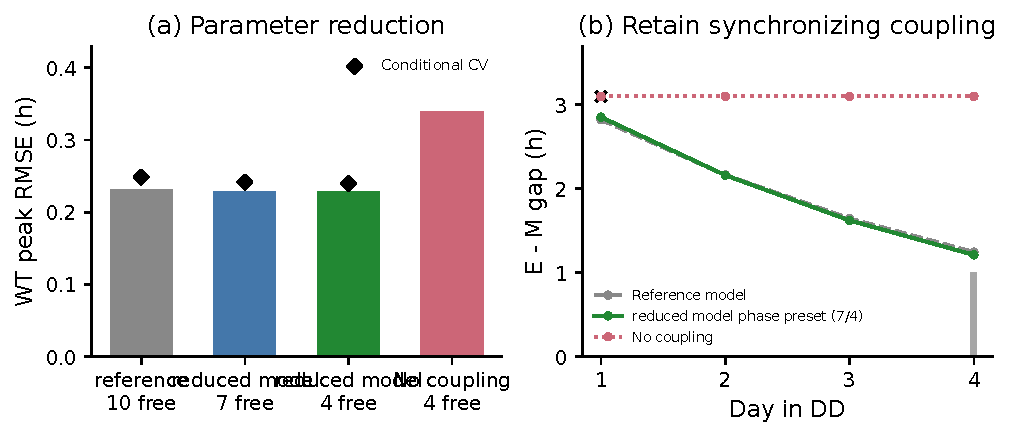
\includegraphics[width=\textwidth]{figure/report/reduction_and_dd.pdf}
\caption{(a) All-data paired peak errors (bars) and conditional CV
(diamonds). (b) Simulated LD12-to-DD gaps. The black cross is the
DD1 calibration target; the thick grey segment marks the assumed
DD4 acceptable gap range 0--1\,h. Removing $\kappa$ preserves the
gap, even though the stationary LD orbits lock.}
\end{figure}

During DD, $L=S=0$, so Eq.~\eqref{eq:mean} becomes
\begin{equation}
\dot m=\omega,\qquad \dot\delta=-2\kappa\sin\delta.
\end{equation}
For $|\delta_0|<\pi$, the solution is
\begin{equation}
\tan\!\frac{\delta(t)}{2}
 =\tan\!\frac{\delta_0}{2}\exp[-2\kappa(t-t_0)].
\label{eq:DD}
\end{equation}
The small-gap relaxation time at the phase preset is
$1/(2\kappa)\simeq80.4$\,h. At $\kappa=0$, the phase difference is
constant. The no-coupling fit therefore cannot reproduce DD convergence.

\begin{center}
\begin{tabular}{rrrr}
\toprule
DD day & Reference model gap & reduced model gap & No-coupling gap\\
\midrule
1 & 2.823 & 2.853 & 3.100 \\
2 & 2.164 & 2.162 & 3.100 \\
3 & 1.646 & 1.623 & 3.100 \\
4 & 1.246 & 1.213 & 3.100
\\
\bottomrule
\end{tabular}
\end{center}

The reduced model DD4 gap remains about 1.21\,h, above the trial bound.
Moreover, $\dot m=\omega$ preserves the mean phase inherited at transfer.
When the gap closes, both peaks approach that inherited mean timing,
not an independently selected CT14. The DD4 common phase reported in
the manuscript was not included in the fitting loss.

The daylength-dependent reference lag also cannot simply be discarded.
With $F=0$ at $P\leq9$, a constant lag and a floor no higher than 9\,h
make the P=9 WT peak and the P=12 PDF-null peak differ by 3\,h.
Their approximate targets, ZT10 and ZT15, differ by 5\,h.
A lag transition or a different reference mechanism is required.
This argument constrains the reference form; it does not establish
that the fly implements the fitted empirical rule.

\clearpage
\section{Sensitivity to the raw observation model}
\label{sec:raw}

The raw-data comparison profiles a periodic transcriptional waveform
against paired M/E mean fractions at each sampled ZT.
For oscillator phase $\phi$, let $u=\phi-\pi$ and
\begin{equation}
H(\phi)=b+(1-b)A
   \exp\!\left[(\cos u-1)c(1+s\sin u)\right].
\end{equation}
Baseline $b$, amplitude $A$, concentration $c$ and skew $s$ are
profiled for each population and condition. With $c>0$ and $|s|<1$,
the global maximum occurs at $u=0$; there is no additional free
observation phase. The comparison retains eight nuisance parameters
per condition, 88 over the 11 conditions.

\begin{center}
\begin{tabular}{lrrr}
\toprule
Architecture & Free clock parameters & Phase preset SSE & Raw-refit SSE\\
\midrule
reference & 10 & 374.167 & 311.443 \\
reduced model (seven free) & 7 & 385.792 & 307.945 \\
reduced model (four free) & 4 & 385.792 & 309.719
\\
\bottomrule
\end{tabular}
\end{center}

The weighted in-sample SSE uses the paired M/E mean covariance plus
an assumed discrepancy variance $(0.03)^2$ for each fraction.
It is a Gaussian mean-error criterion, not a binomial count likelihood,
reduced $\chi^2$, AIC or raw-data CV. The joint optimization also includes
KO/DD/locking penalties; the table shows only the waveform component.
All profiled curves and both reduced raw optimizers converge.

\begin{figure}[h]
\centering
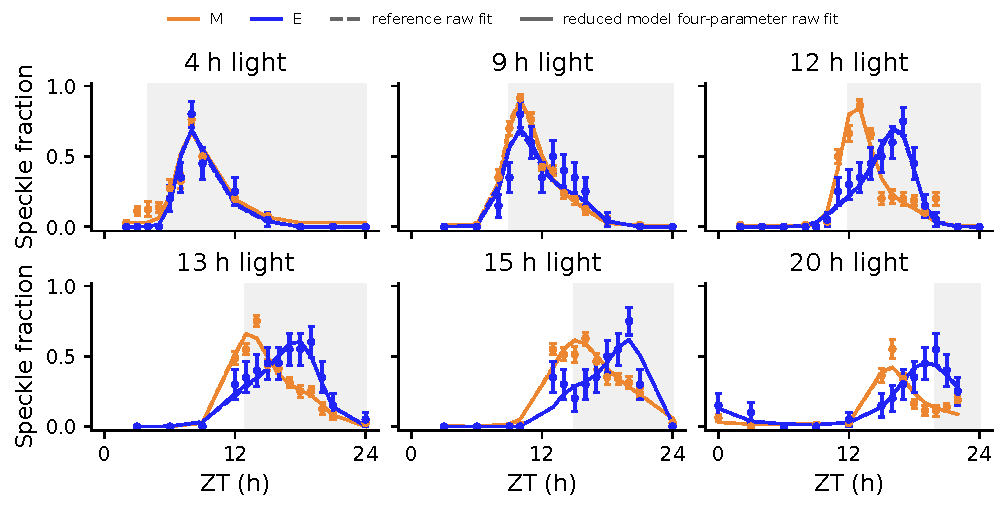
\includegraphics[width=\textwidth]{figure/report/raw_waveforms.pdf}
\caption{Six representative photoperiods, using joint raw clock fits.
Points show mean fractions with SEM; dashed lines are the ten-parameter
reference fit and solid lines the four-parameter reduced model fit. Shading marks
darkness. Lines connect predicted values at sampled ZT for display.
Both architectures retain identical observation flexibility.}
\end{figure}

Refitting reduces the compact waveform error to a value close to the
historical ten-parameter raw fit. Small differences between local fits
with different starts/budgets are not evidence that one architecture
is statistically better. The raw-fit clock parameters differ from the
phase preset in Table~\ref{tab:params}. The saved paired-brain reconstruction,
blank/zero handling and column pairing still require experimental
confirmation; no source workbook was modified by this study.

\clearpage
\section{Interpretation, limitations and next experiments}

The symmetry constraint removes an apparent distinction between M and E
PDF magnitudes that is not needed to explain the tested stationary peaks.
It does not show that biological receptor sensitivity is identical.
Likewise, $q=1$ and $\chi=0$ are economical effective descriptions,
not measurements of the shape and timing of PDF release.

The simplest useful interpretation has three components: a shared
photoperiod-dependent reference supplies the common timing; an effective
PDF-associated drive separates the phases; synchronization pulls them
together, including in DD. This framework preserves two neuron populations
and their distinct PDF/PDFR perturbation responses. Its parameters do not
uniquely identify molecular or synaptic pathways.

\begin{tcolorbox}[colback=orange!4,colframe=orange!50!black,boxrule=0.5pt,
 title=Remaining limits]
\begin{itemize}
\item \textbf{Season sensing is supplied, not inferred.}
$P$ enters the reference and activation directly. Fixed 9/15-hour
landmarks and the extra rounded constants are data-informed.
\item \textbf{DD relaxation is incomplete.}
The candidate overpredicts the DD4 gap and does not select the
reported common phase near CT14.
\item \textbf{Transient protocols are unresolved.}
The earlier adapting/intensity-gated pulse trials do not jointly
explain LD, DD and all pulse targets. Binary-light reduced model is not a new
intensity-dependent pulse fit.
\item \textbf{Amplitude is an observation fit.}
The phase dynamics do not predict transcriptional amplitude or
the disappearance of rhythmicity.
\item \textbf{Statistical uncertainty remains provisional.}
Phase targets use the stored earlier bootstrap summaries, rather
than the manuscript's newer nested estimator; several error scales
are assumed and fixed-constant selection uses the same data.
\end{itemize}
\end{tcolorbox}

The next useful analysis is an identifiability study: profile
$K,\gamma,\kappa$ and the three proposed fixed constants with broader
starts, retaining the DD and knockout constraints. That would show
whether distinct parameter combinations trade light attraction against
separating drive and synchronization.

For a stronger experimental test, specify the reduced model and its
anchors before collecting intermediate photoperiods, especially near
the activation transition. Measure complete DD trajectories and the
common phase, rather than only DD1/DD4 gap summaries. Independent PDF
release or activity measurements would test the symmetric release rule.

A subsequent mechanistic model could replace explicit $P$ with a causal
light-history state. Such a change should be fitted jointly to stationary
LD, DD and pulse data, using the measured experimental initial conditions
and reconciled waveform uncertainty. The present comparison does not
establish that adding that state will improve prediction.

\clearpage
\section{Reproduction and sharing}

The numerical inputs are the saved simplification results and the earlier
reference observation/raw-fit archives. Figure and table values are generated
from those files rather than transcribed by hand.
Their checksums are in \path{figure/report/manifest.json}.
The saved comparison results and validation summaries are supplied in
\path{out/model_comparison/}.

Build the report from the repository root without refitting:
\begin{lstlisting}
uv sync
uv run python code/build_report_assets.py
mkdir -p output/pdf
latexmk -pdf -interaction=nonstopmode -halt-on-error \
  -output-directory=output/pdf dual_oscillator_model_note.tex
\end{lstlisting}
The PDF is standalone. The accompanying source ZIP contains this
LaTeX file and all vector figures/table inputs; it compiles without
Python or access to the raw workbooks.

The compact phase preset can be evaluated as follows:
\begin{lstlisting}
PYTHONPATH=code uv run python - <<'PY'
import phase_model as model
print(model.periodic_summary(12)["peaks"])
print(model.dd_transfer())
PY
\end{lstlisting}
To access the conservative seven-parameter candidate, the saved
\texttt{linear\_window} entry is decoded into the reference equations:
\begin{lstlisting}
PYTHONPATH=code uv run python - <<'PY'
import json
import reference_phase_model as model
r = json.load(open("out/model_comparison/results.json"))
p = model.Params(**r["results"]["linear_window"]["parameters"])
print(model.periodic_summary(12, p, "separate_release",
                             days=60)["peaks"])
PY
\end{lstlisting}

\texttt{README.md} gives the constrained-fit, conditional CV,
raw-refit and audit commands. The full test suite has 33 passing tests,
including frozen-version checksums, genotype constraints, the exact
mean--gap vector field, the positive-velocity domain, WT invariance,
and compact LD/DD integration agreement. Checks do not establish
global optimality or resolve the experimental limitations above.

\begin{thebibliography}{9}
\bibitem{project}
Seasonal-clock project manuscript (October 2026),
\emph{A plastic transcriptional phase gap encodes seasonal time in
clock neurons}. Unpublished project source with associated Figure 4
workbooks; experimental and protocol context as documented in the reference note.
\bibitem{v02}
Qin, S. (2026).
\emph{An Alternative Dual-Oscillator Model of Seasonal Transcriptional
Timing in Drosophila}. Project modelling note, version 0.2.
Ten-parameter separate-release baseline frozen at Git tag
\texttt{model-reference}.
\end{thebibliography}

\end{document}
